\documentclass[aagreenthesis]{subfiles}
\begin{document}
\chapter{Structure-Property in the \nfour{} Homologous Series of Molecules}

Now that the existance of the \smcpalpha{} and \smcapa{} phase have been put on
a firm footing, we can extend this study to a broad category of molecules that
share the same core, but have variations in the tail length. Our previous study
focussed on \nfour{}, with a tail length of n=14 carbons. Inspired by
previous studies by the Dublin
group\cite{SreenilayamSpontaneoushelixformation2016,SreenilayamDevelopmentferroelectricitysmectic2017,VijInvestigationheliconicalsmectic2019},
where the n16 and n18 compounds were studied and a helical phase was tentatively
determined based on periodicities of around \SI{5}{\nano\metres} see in atomic
force microscopy images.

With the ability to directly probe the periodicity of these compounds with
carbon K-edge resonant X-ray, we have the ability to provide direct evidence for
helical phases in these molecules. The high-resolution provide by RSoXS
additionally allows for a rich study of structure-property relationships, where
the nature of the helical phase can be connected to the tail-length.

Interest in the \nfour{} series of molecules is not confined to the discovery of
helicity. The additional discovery of a bent-core de Vries like phase is also a
motivating interest for study of this series. 

This chapter is organized under discussion of these two phases. First the
helical, smectic \smcpalpha{} is presented and discussed for the n12, n14, and n16 molecules.
Then the bent-core de Vries phase is presented and discussed for this series.

\section{The \smcpalpha{} Phase: Smectic Chirality Beyond the B2 Phase}


\section{The bent-core de Vries phase}

The evidence for a bent-core de Vries phase in \nfour{} will be briefly
reviewed. It is worth noting that the question of ``what is a de Vries phase''
is not settled, even for the simpler phases of rod-shaped molecules, see Jan
Lagerwall's thesis\cite{jansThesis} for an excellent history and discussion of
de Vries phases in the calamitic paradigm. For the purposes of this thesis, we
take the broadest view of a de Vries: it is a tilted phase with no long-range
order present in the tilt order parameter.

Even this broad definition is not free from ambiguity--- what entails long-range
order, and does it matter how the escape from long-range order is achieved? We will also see in this Chapter that the de Vries phase can be
suppressed quite easily by a strong-alignment layer.



To satisfy our definition, we must prove two things about the phase under
investigation to say it is a de Vries bent-core phase. First, it must be tilted.
Second, it must have no long-range order present. Both of these facts are very
difficult to establish in a postive manner, as there is no `smoking-gun'
evidence for either.

We claim that \nfour{} is tilted for the following reasons: the smectic layer spacing is
significantly less than the extended molecular length; the lower temperature
phases are proven to be chiral (therefore tilted), and there is no observed
smectic layer-contraction observed on cooling, which would be expected for an
orthogonal$\rightarrow$ tilted phase transition; and there is no measured change in the birefringence which would be predicted from an orthogonal phase to the
helical \smcpalpha{} (confirmed from RSoXS). All of these facts together suggest
that the highest temperature smectic phase of \nfour{} is tilted.

To see that there is no long-range order in the tilt order parameter, we can
look at the textures of this phase and observe that they look orthogonal-- they
have the clean lines of a focal conic SmA phase. This
is neccesary but not sufficient, as other phase-- such as the \smcapa{} phase --
can also appear to be orthogonal, yet have a definite anti-clinic long range
order. This anti-clinic order (and other, more exotic long helical ordering of
the tilt order paramter) would show up in resonant x-ray scattering. The fact
that the resonant x-ray scattering shown in \autoref{fig:pal30:rsoxs} reveals
zero periodic structure for \nfour{} confirms that the tilt order in the Sm1
phase has no long-range order.

The actual way that this is achieved is still ambigious. The simplest model,
where the molecules are rotating freely around a cone whose opening angle is
set by the molecular tilt seems unlikely from simple enthalpic space-filling
arguments which would seem to exclude a model where neighboring molecules can be
pointing in completely opposite directions with no energy cost. On the surface,
this seems to be false, but close observation of the c-director flucuations
that occur in freely-suspended-films shows that at the molecular level the
c-director can easily be flucuating with $\pi$-rotations measured against
neighboring molecules, so we cannot rule out this type of behaviour purely on
enthalpic concerns.\todo{need to find de gennes/noels argument for this} This is
fluid-like model, where the molecules are actively rotating with no regard for their
neighbors space.

By including these enthalpic considerations we can build model where short-range order persists, but the size of
these ordered domains is small, and they are randomally distributed such that
an ensemble average of the tilt is zero. This is more of a disordered-crystal
model, where short-range order persists, but is distributed in such a way that the
macroscopic order parameter is still zero-- much like the example of a cooled
ising model developing local ferroelectric ordering of spins, even though the
total magnetization remains zero. 

Regardless of how this long-range tilt order is broken, because these are polar
molecules, we also have to consider the polar-ordering present in any phase.
The way that the polar and tilt interact in the high-temperature de Vries SmA of
\nfour{} is unique to bent-cores.

\begin{figure}[h!]
    \centering
    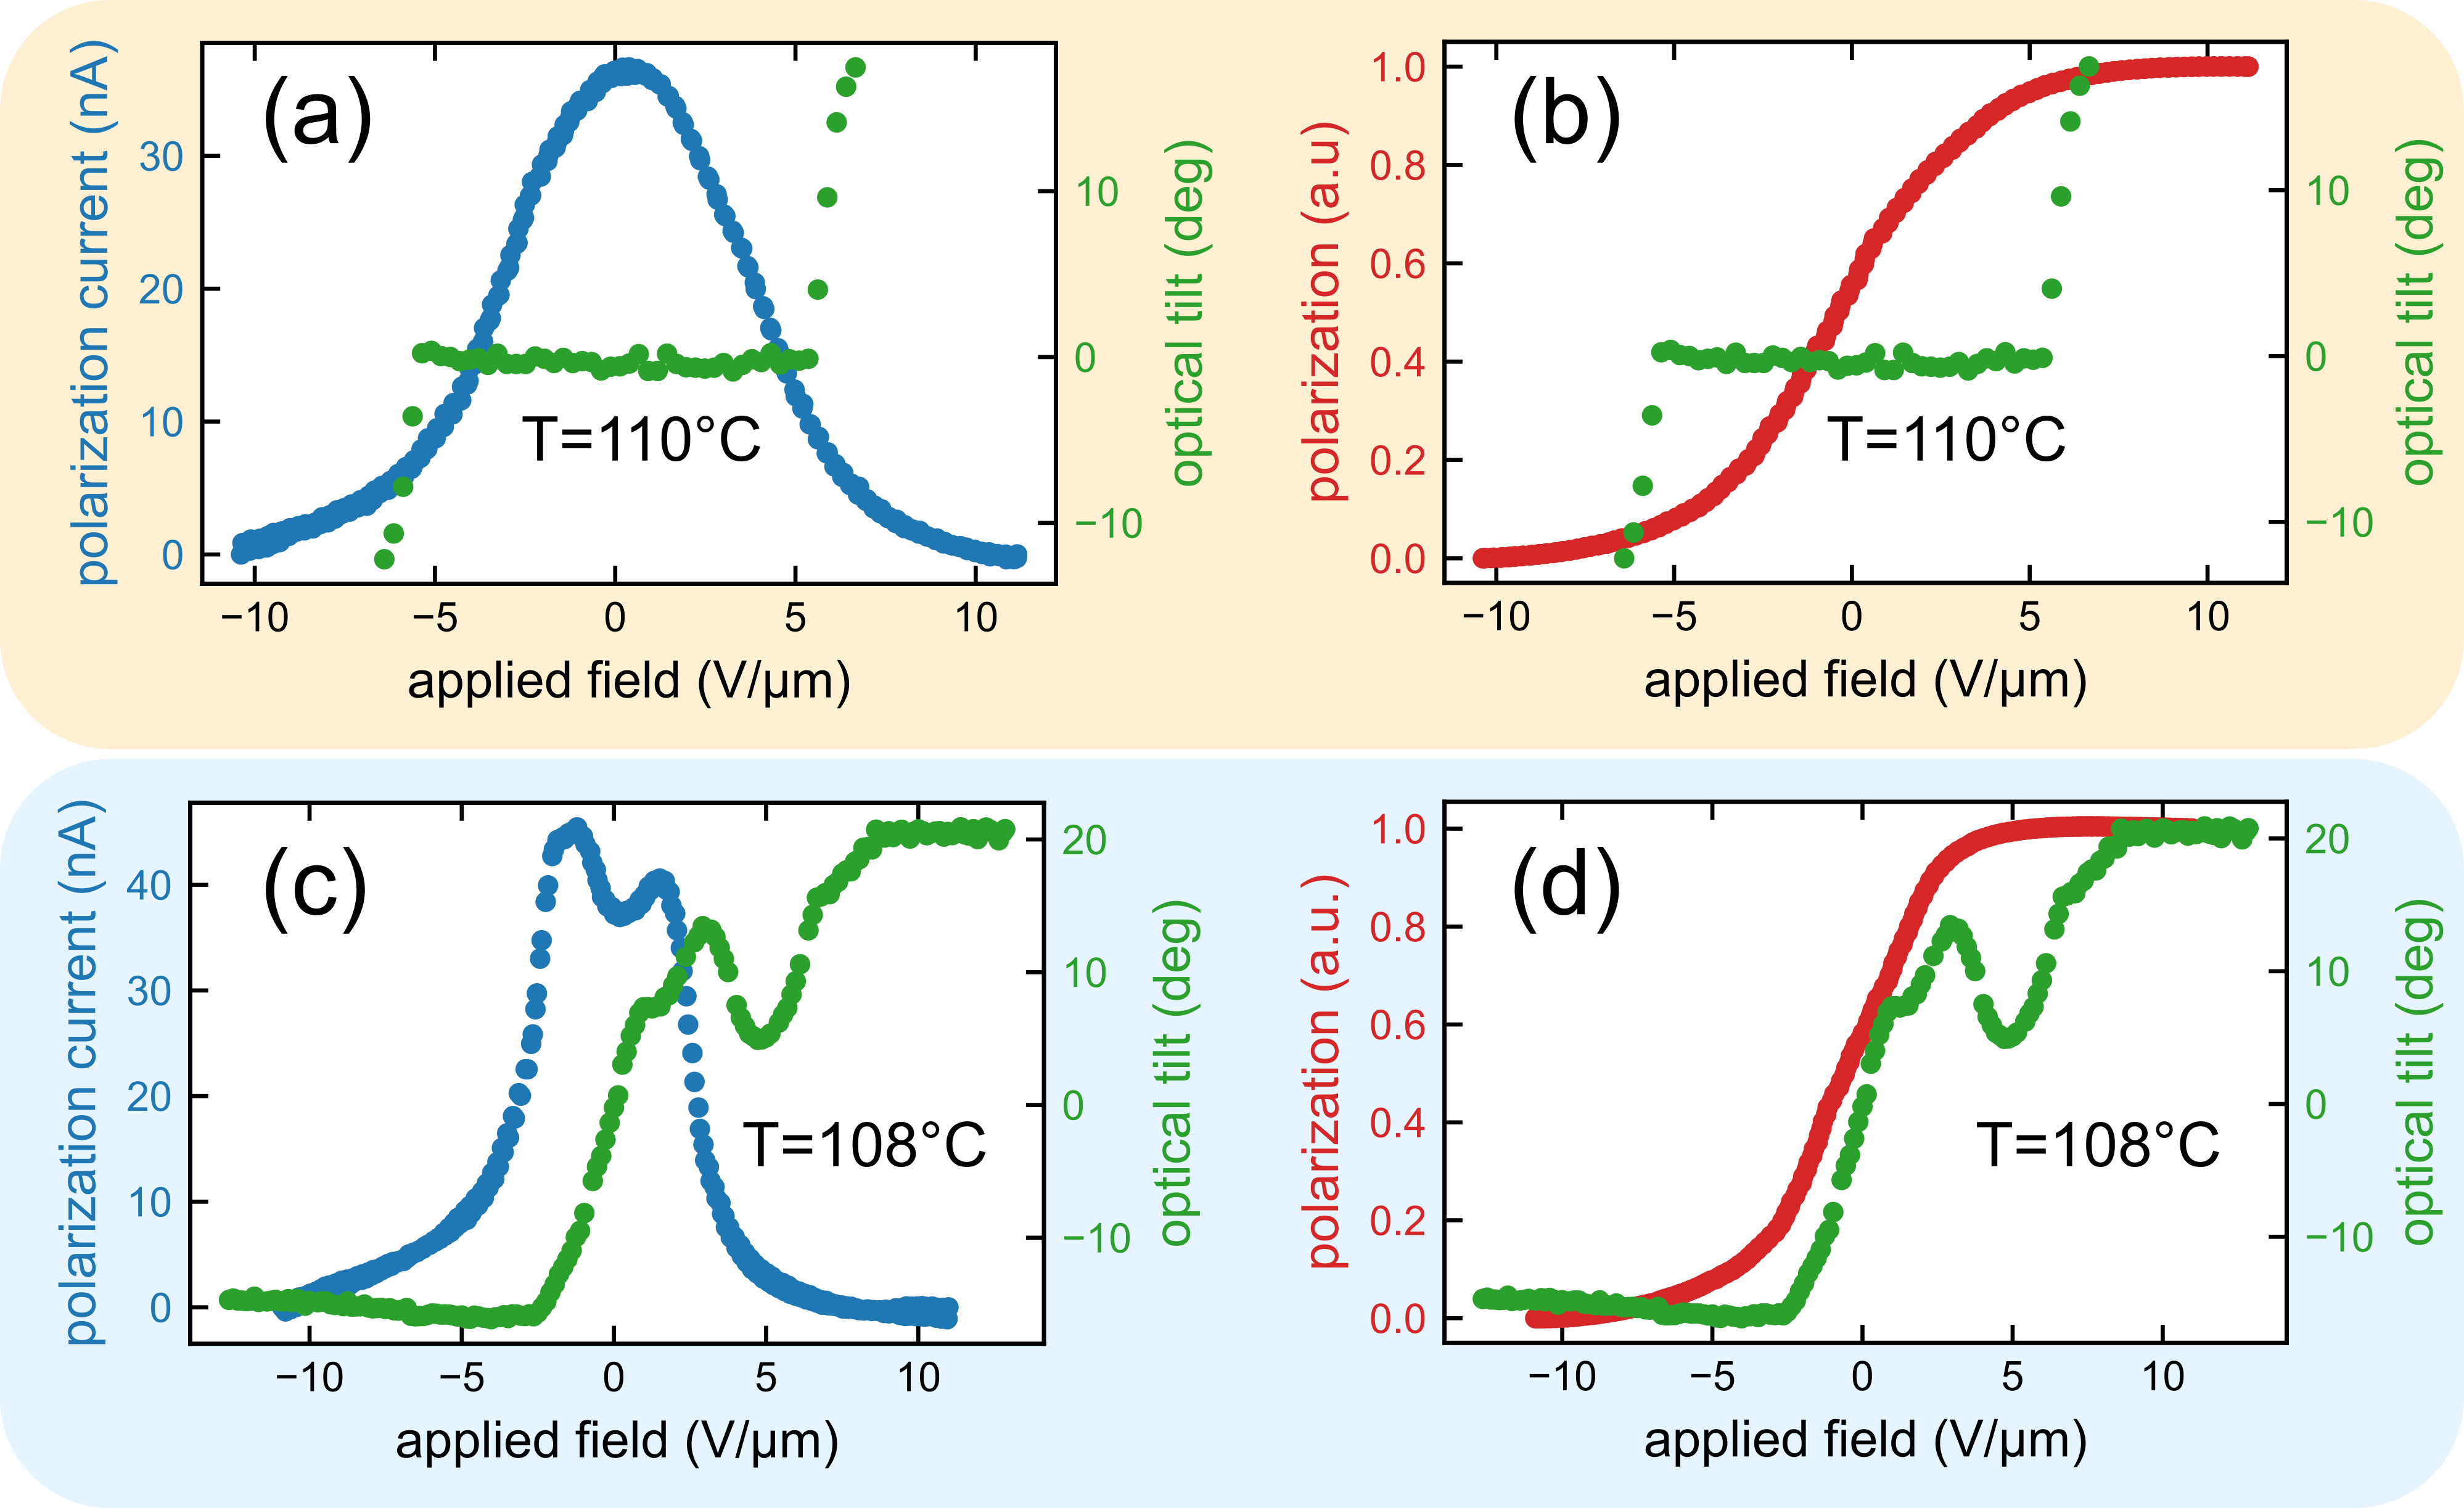
\includegraphics[width=.6\textwidth]{./figs/pal30/prc/PRCvsTilt/PRCVtilt.png}
    \caption{\label{fig:homog:pal30pvt} The polarization current and the optical
    tilt plotted as a function of applied field strength for both the Sm1
(de Vries SmA) (a,b) and the Sm2 (\smcpalpha{}) (c-d). The polarization current
has additionally been integrated to calculate the time-dependant net
polarization. The threshold electric field ($E_\textrm{th}$) required to manifest the tiger-stripes can
be directly read from the green curve denoting the optical tilt (for
T=\SI{110}{\degreeCelsius}, $E_\textrm{th} \approx \SI{5}{\volt\per\micro\metre}$),
and the saturation electric field where the net polarization is no longer
changing ($E_\textrm{sat}$) can be directly
read from the red curve, which denotes the net polarization, (for
T=\SI{110}{\degreeCelsius}, $E_\textrm{sat} \approx \SI{5}{\volt\per\micro\metre}$).
Both $E_\textrm{th}$ and $E_\textrm{sat}$ are plotted in as the inset of
\autoref{fig:threshold}. }
\end{figure}

The polarization current has been integrated to give the net polarization, which
is a direct measure of the ensemble average of the molecular orientation with an
applied electric field. The optical tilt measurements were done by analyzing the
contrast between adjacent stripes\todo{small figure showing this}. In the ground
state, where there is no long-range order present in tilt, the contrast is zero.
At a field whose strength is over some threshold value ($E_\textrm{th}$), the
state transitions into a tilted (therefore chiral) state. The handedness of the
domain sets the tilt direction. This tilt can be directly measured as it is
proportional to the contrast between different handed domains:
\begin{equation}
    \textrm{contrast}\propto \sin(4\theta)
\end{equation}\todo{check this}.
Barring pathological examples, \textit{any} alignment, orientation, or movement
of the molecular long axis will show up as the observable seperation of the
texture into chiral domains. 


With some unique exceptions\cite{michi}\todo{cite michi}
most bent-core systems have the tilt and
polarity strongly coupled: where one moves, the other follows. Through symmetry,
this can be expressed as the condition that rotations around the molecular long
axis are forbidden: to transition to different states, the molecule must rotate
around the smectic layer normal, confined to the tilt-cone.
\autoref{fig:homog:pal30pvt} clearly shows that the movement of the polar
director (rotations around the long axis of the molecule) is decoupled from the
movement of the c-director (rotations around the smectic layer normal on the
tilt-cone).\todo{small inline figure of this} The polarization first saturates
before there is any detectable movement of the tilt-director. The previous
examples of this occuring in bent-cores required pulse-engineering the applied
voltage,
where a very large, fast voltage needed to be applied to see rotations around
the long axis of the molecule. \nfour{} is the first molecule where the polar
and tilt order have been confirmed to be decoupled in its ground-state.

This decoupling results in 
an important distinction because, unlike their calamitic cousins, these
bent-core molecules are not inherently chiral. They are only develop chirality
once they pack into phases. they require tilt and smectic ordering
before the mirror-symmetry breaking required for chirality is achieved. They
also require that the tilt and polar order are strongly coupled--free rotations
around the long-axis result in a return of mirror-symmetry and the chirality of
the phase is broken. In contrast to the calamtics, who merely have to `discover'
their own inherent chirality once a field is applied (for instance, in the
electroclinic effect), the bent-cores must spontaneously create their own. This
is not a new discovery, the B2 phases\cite{link_spontaneous_1997} have long been
known to develop spontaneous chirality on cooling from an achiral phase. This is
the first discovery of field-activated chirality in a bent-core system, where
chirality is induced at a certain voltage, but then returns to an achiral ground
state when the voltage is removed.


The closest thing to a developed model for this phase is the Landau-de Gennes
model put forth by Eremin et al.\cite{eremin2008electrically} where they
discovered an electro-clinic analog in a hockey-stick compound. 
\todo{get and show the molecule}
\begin{figure}
    \centering
    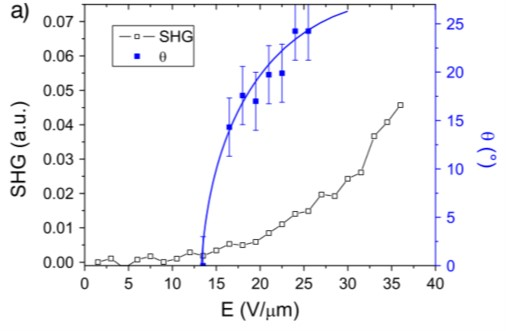
\includegraphics[width=\textwidth]{./figs/pal30/fromPapers/tiltVfield.jpg}
    \caption{\label{fig:achiralTilt} Experimental data for `hockey-stick'
    compound studied by Eremin et al.\cite{eremin2008electrically} Note, the threshold for optical tilt. The lines guide the only.}
\end{figure}
Broadly, their model describes an orthogonal bent-core phase where the polar
director is free to move. On application of an electric-field, the polarization
of the molecules orients. An enthalpic\todo{check this with ed} phase transition
is then driven by excluded-volume interactions, where the molecules can pack
more efficiently by tilting. 

This interaction is described by the following Landau-de Gennes free energy:

\begin{multline}
    f(P,\theta,T,E) = \overbrace{\left(a_0(T-T_\theta)\theta^2+b\theta^4+c\theta^6
    \right)}^{f_\theta}\\
    + \underbrace{\left( \alpha_0(T-T_P)P^2+\beta P^4 + \gamma P^6 -PE
            \right)}_{f_P} +\underbrace{\left(
    -\Gamma (P \theta)^2 \right)}_{f_{\theta P}}
\end{multline}

Though this model was originally formulated to describe the transition from an
orthogonal phase to a tilted one, we can adapt it to our bent-core de Vries
phase by changing the interpretation of $\theta$ from the molecular tilt to the
optical tilt.

Though this model succesfully captures the overall nature of the
electically-driven onset of chirality in the bent-core de Vries phase, where the
molecules first orient their polar directors to the field, and on the
achievement of total polar alignment, an optical tilt develops, it leaves much
to be desired. Because this model does not demand details of the
microscopic interactions that lead to the observed transition, there is an abundance of
fitting parameters that will lead to overfitting and the model loses most of its
predictive power.

Because of this, efforts must be undertaken to develop a microscopic model of
this de Vries phase.

\subsection{Textures of bent-code de Vries phase}

\begin{figure}[h!]
    \centering
    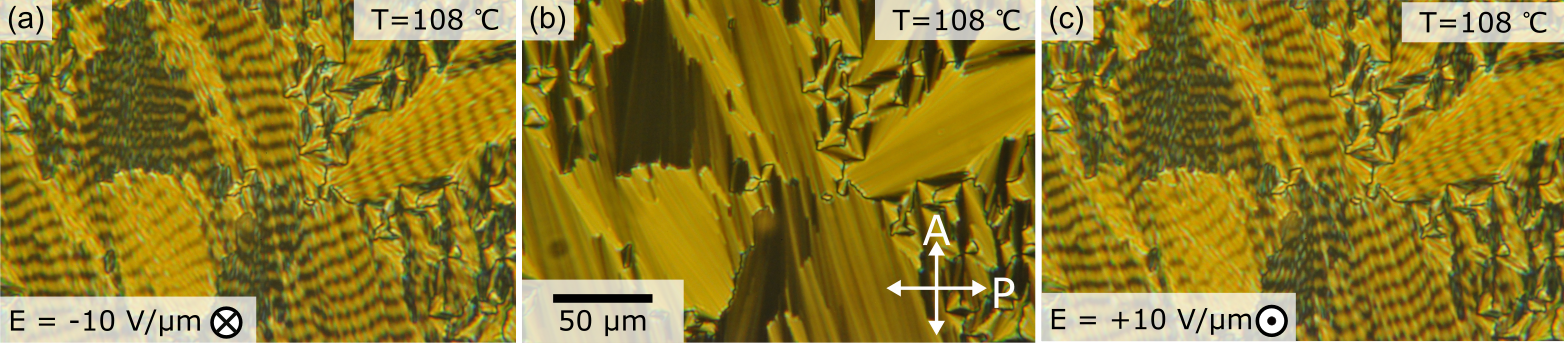
\includegraphics[width=.8\textwidth]{figs/pal30/textureSM2/sm1Textures100.png}
    \caption{\label{}}
\end{figure}


\subsection{Electro-optics of bent-core de Vries phase}
text
\begin{figure}[h!]
    \centering
    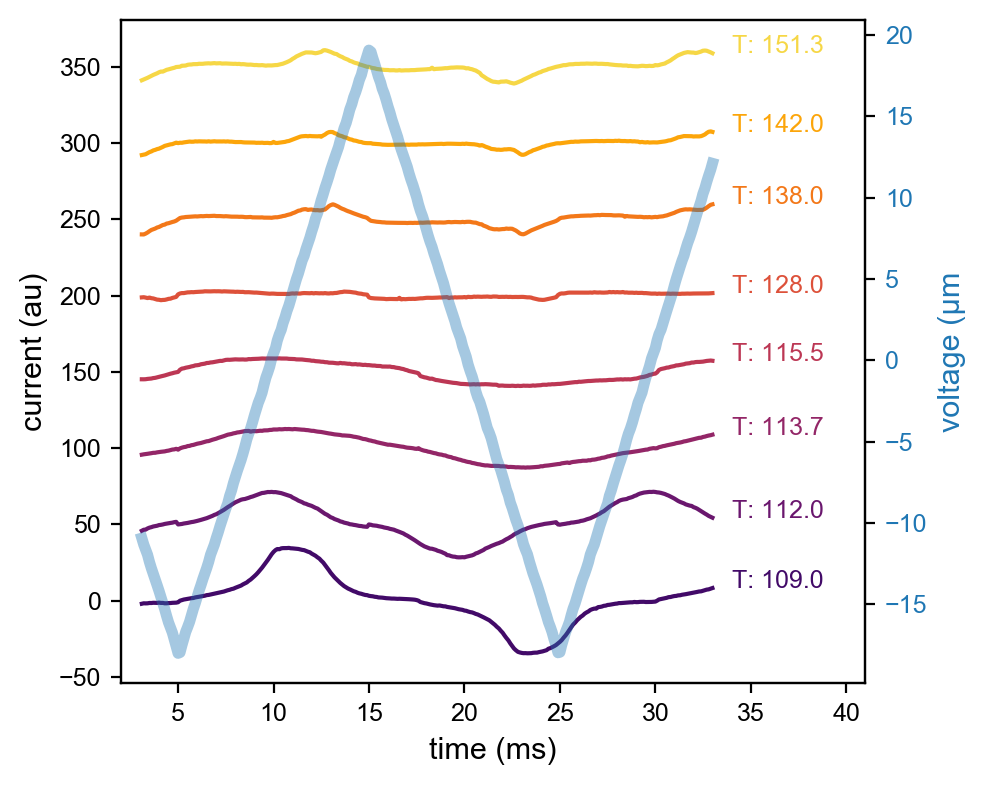
\includegraphics[width=.8\textwidth]{figs/pal30/prc/spacedSm1PRC.png}
    \caption{\label{}}
\end{figure}
text

\begin{figure}[h!]
    \centering
    \includegraphics[width=.8\textwidth]{figs/pal30/prc/3dplot-sm1.png}
    \caption{\label{}}
\end{figure}
text

\subsection{X-ray analysis of bent-core de Vries phase}

\begin{figure}[h!]
    \centering
    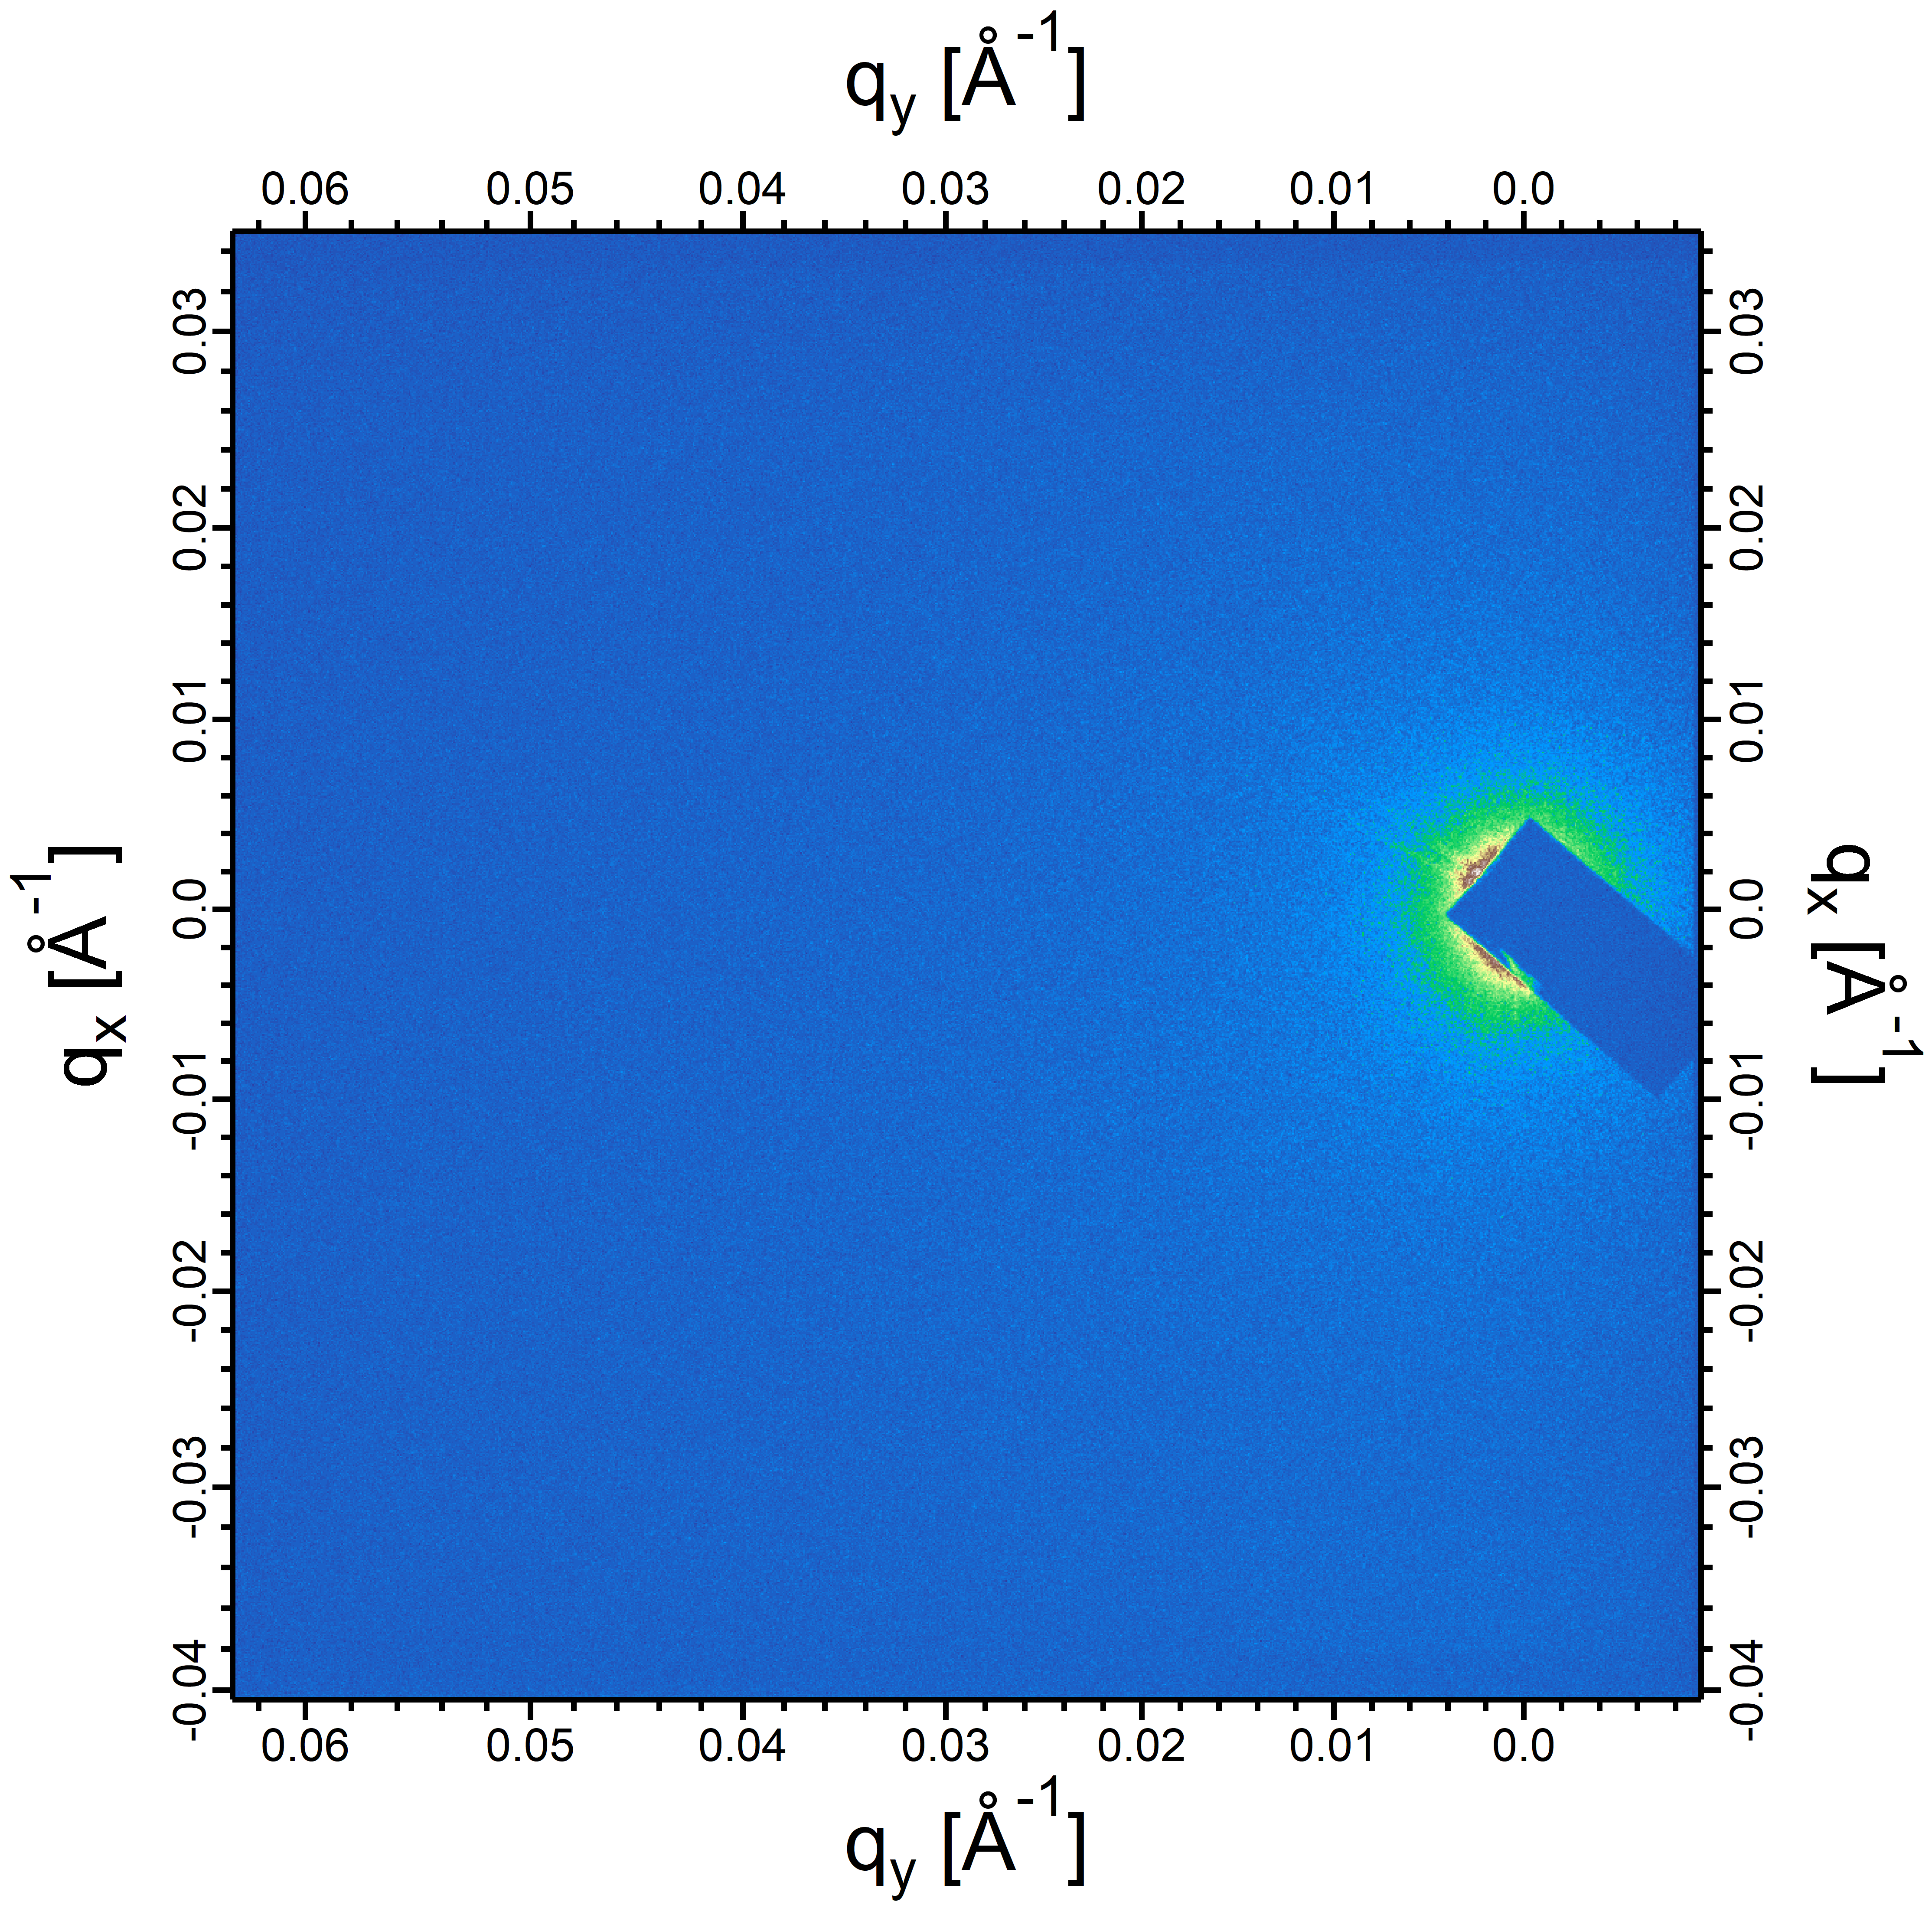
\includegraphics[width=.8\textwidth]{figs/pal30/xraysm1/rsosxSmaT113-modified.png}
    \caption{\label{}}
\end{figure}


\begin{figure}[h!]
    \centering
    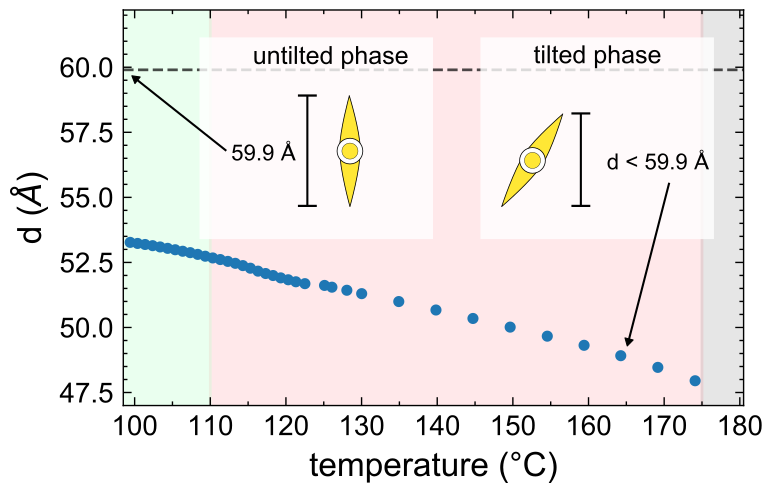
\includegraphics{figs/pal30/xraysm1/sm1-saxs-annote.png}
    \caption{\label{}}
\end{figure}




\section{Discussion for the bent-core de Vries phase}
\begin{figure}[h!]
    \centering
    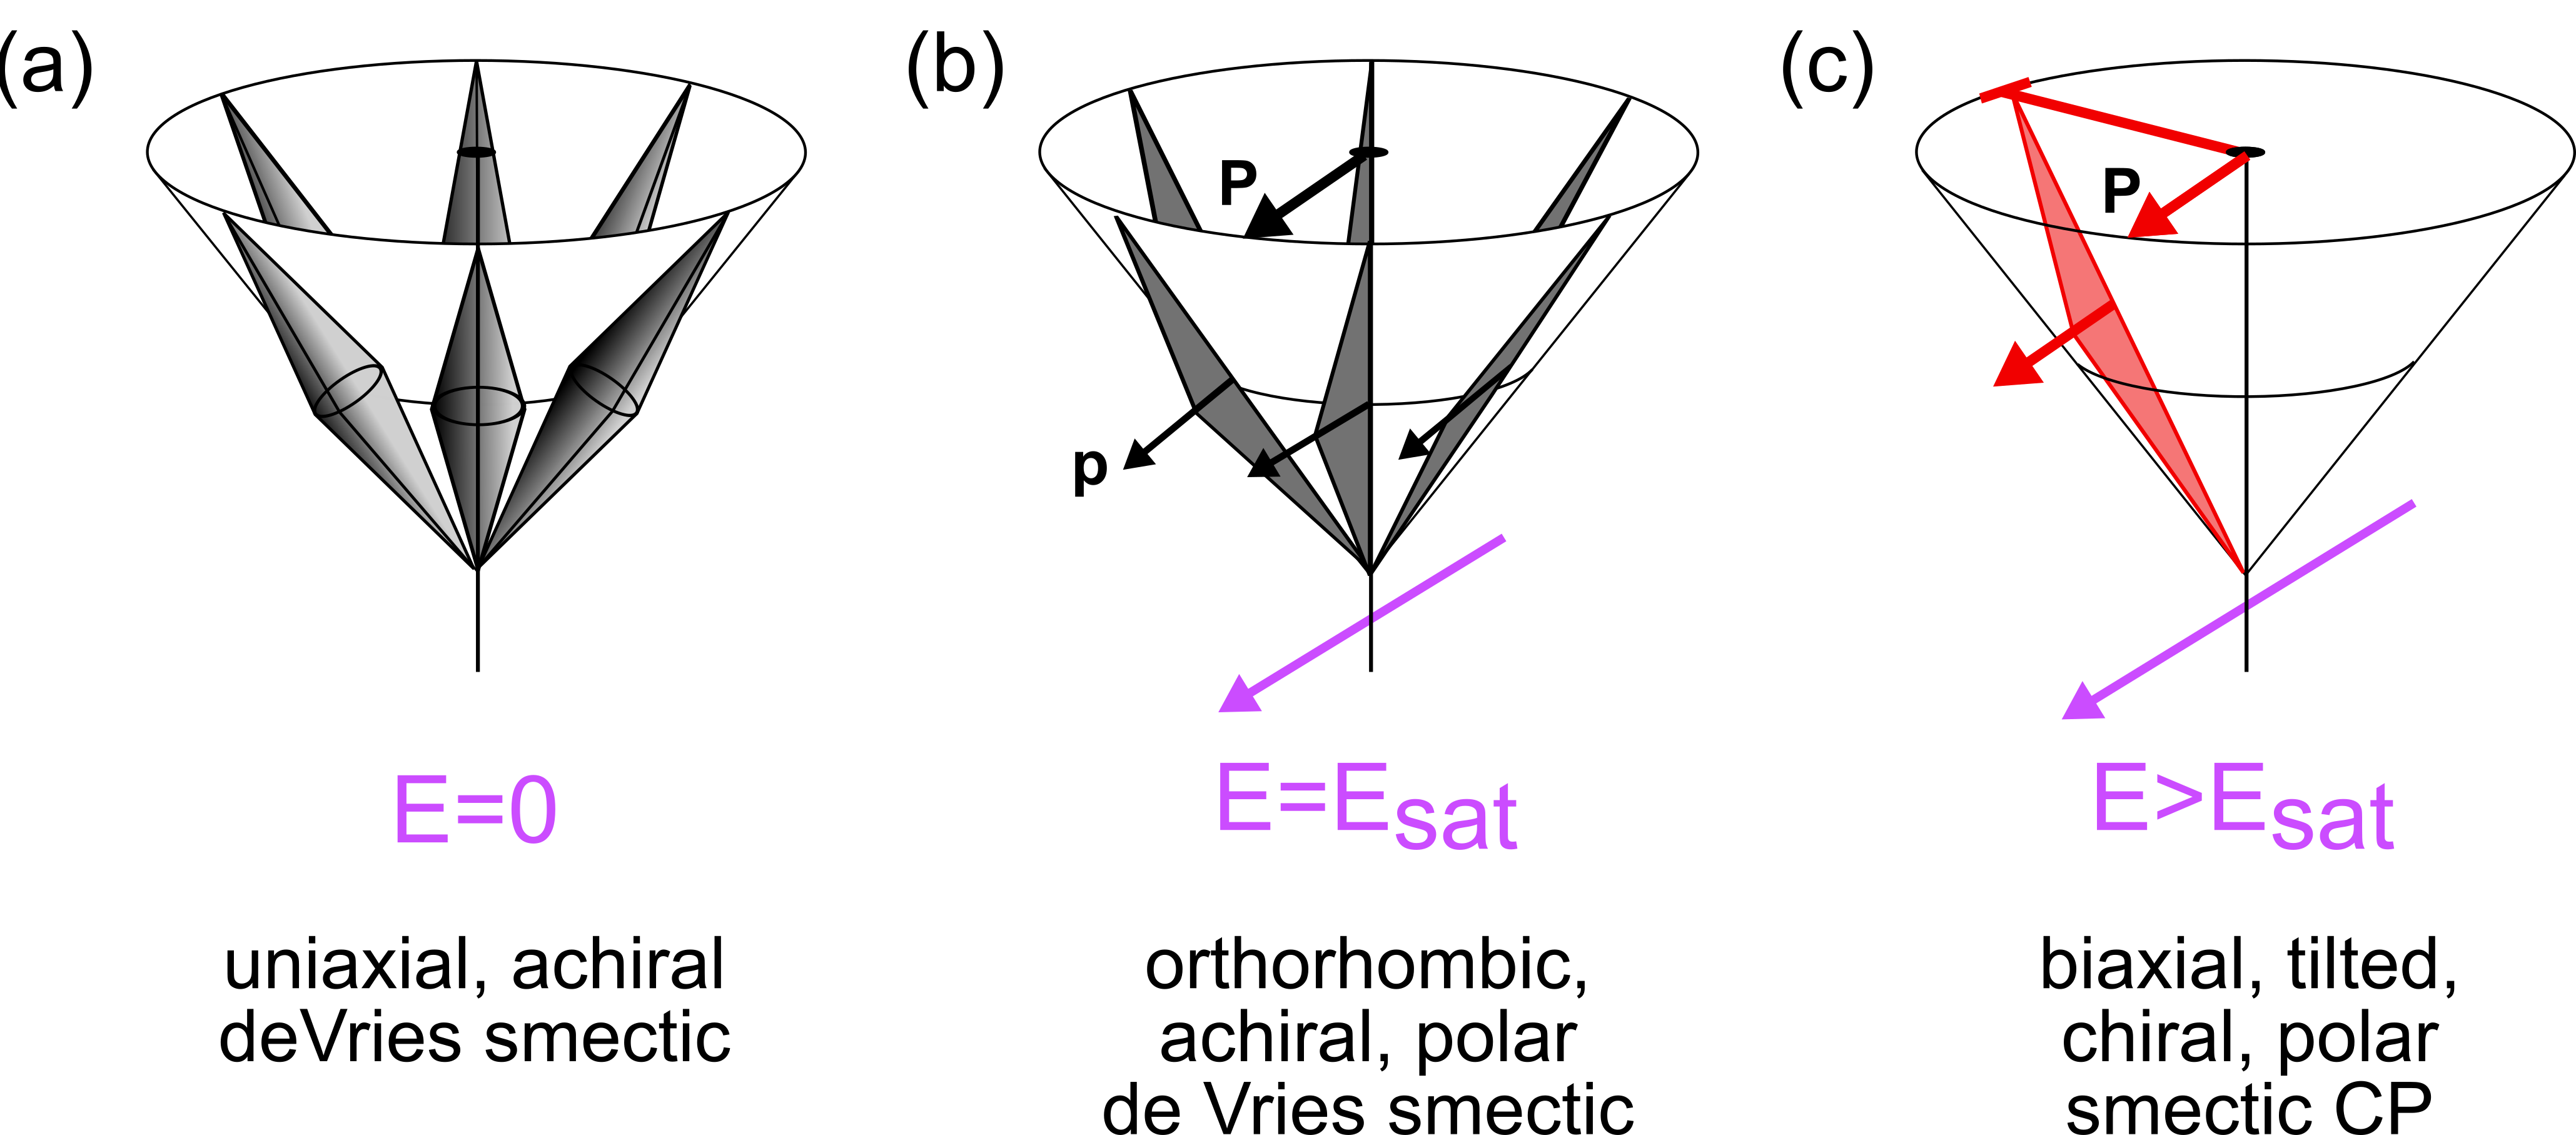
\includegraphics{figs/pal30/deVries/dvAlign.png}
    \caption{\label{}}
\end{figure}




\end{document}


